% Options for packages loaded elsewhere
\PassOptionsToPackage{unicode}{hyperref}
\PassOptionsToPackage{hyphens}{url}
\PassOptionsToPackage{dvipsnames,svgnames*,x11names*}{xcolor}
%
\documentclass[
]{krantz}
\usepackage{lmodern}
\usepackage{amssymb,amsmath}
\usepackage{ifxetex,ifluatex}
\ifnum 0\ifxetex 1\fi\ifluatex 1\fi=0 % if pdftex
  \usepackage[T1]{fontenc}
  \usepackage[utf8]{inputenc}
  \usepackage{textcomp} % provide euro and other symbols
\else % if luatex or xetex
  \usepackage{unicode-math}
  \defaultfontfeatures{Scale=MatchLowercase}
  \defaultfontfeatures[\rmfamily]{Ligatures=TeX,Scale=1}
\fi
% Use upquote if available, for straight quotes in verbatim environments
\IfFileExists{upquote.sty}{\usepackage{upquote}}{}
\IfFileExists{microtype.sty}{% use microtype if available
  \usepackage[]{microtype}
  \UseMicrotypeSet[protrusion]{basicmath} % disable protrusion for tt fonts
}{}
\makeatletter
\@ifundefined{KOMAClassName}{% if non-KOMA class
  \IfFileExists{parskip.sty}{%
    \usepackage{parskip}
  }{% else
    \setlength{\parindent}{0pt}
    \setlength{\parskip}{6pt plus 2pt minus 1pt}}
}{% if KOMA class
  \KOMAoptions{parskip=half}}
\makeatother
\usepackage{xcolor}
\IfFileExists{xurl.sty}{\usepackage{xurl}}{} % add URL line breaks if available
\IfFileExists{bookmark.sty}{\usepackage{bookmark}}{\usepackage{hyperref}}
\hypersetup{
  pdftitle={Beyond Multiple Linear Regression},
  pdfauthor={Paul Roback and Julie Legler},
  colorlinks=true,
  linkcolor=Maroon,
  filecolor=Maroon,
  citecolor=Blue,
  urlcolor=Blue,
  pdfcreator={LaTeX via pandoc}}
\urlstyle{same} % disable monospaced font for URLs
\usepackage{color}
\usepackage{fancyvrb}
\newcommand{\VerbBar}{|}
\newcommand{\VERB}{\Verb[commandchars=\\\{\}]}
\DefineVerbatimEnvironment{Highlighting}{Verbatim}{commandchars=\\\{\}}
% Add ',fontsize=\small' for more characters per line
\usepackage{framed}
\definecolor{shadecolor}{RGB}{248,248,248}
\newenvironment{Shaded}{\begin{snugshade}}{\end{snugshade}}
\newcommand{\AlertTok}[1]{\textcolor[rgb]{0.33,0.33,0.33}{#1}}
\newcommand{\AnnotationTok}[1]{\textcolor[rgb]{0.37,0.37,0.37}{\textbf{\textit{#1}}}}
\newcommand{\AttributeTok}[1]{\textcolor[rgb]{0.61,0.61,0.61}{#1}}
\newcommand{\BaseNTok}[1]{\textcolor[rgb]{0.06,0.06,0.06}{#1}}
\newcommand{\BuiltInTok}[1]{#1}
\newcommand{\CharTok}[1]{\textcolor[rgb]{0.5,0.5,0.5}{#1}}
\newcommand{\CommentTok}[1]{\textcolor[rgb]{0.37,0.37,0.37}{\textit{#1}}}
\newcommand{\CommentVarTok}[1]{\textcolor[rgb]{0.37,0.37,0.37}{\textbf{\textit{#1}}}}
\newcommand{\ConstantTok}[1]{\textcolor[rgb]{0,0,0}{#1}}
\newcommand{\ControlFlowTok}[1]{\textcolor[rgb]{0.27,0.27,0.27}{\textbf{#1}}}
\newcommand{\DataTypeTok}[1]{\textcolor[rgb]{0.27,0.27,0.27}{#1}}
\newcommand{\DecValTok}[1]{\textcolor[rgb]{0.06,0.06,0.06}{#1}}
\newcommand{\DocumentationTok}[1]{\textcolor[rgb]{0.37,0.37,0.37}{\textbf{\textit{#1}}}}
\newcommand{\ErrorTok}[1]{\textcolor[rgb]{0.14,0.14,0.14}{\textbf{#1}}}
\newcommand{\ExtensionTok}[1]{#1}
\newcommand{\FloatTok}[1]{\textcolor[rgb]{0.06,0.06,0.06}{#1}}
\newcommand{\FunctionTok}[1]{\textcolor[rgb]{0,0,0}{#1}}
\newcommand{\ImportTok}[1]{#1}
\newcommand{\InformationTok}[1]{\textcolor[rgb]{0.37,0.37,0.37}{\textbf{\textit{#1}}}}
\newcommand{\KeywordTok}[1]{\textcolor[rgb]{0.27,0.27,0.27}{\textbf{#1}}}
\newcommand{\NormalTok}[1]{#1}
\newcommand{\OperatorTok}[1]{\textcolor[rgb]{0.43,0.43,0.43}{\textbf{#1}}}
\newcommand{\OtherTok}[1]{\textcolor[rgb]{0.37,0.37,0.37}{#1}}
\newcommand{\PreprocessorTok}[1]{\textcolor[rgb]{0.37,0.37,0.37}{\textit{#1}}}
\newcommand{\RegionMarkerTok}[1]{#1}
\newcommand{\SpecialCharTok}[1]{\textcolor[rgb]{0,0,0}{#1}}
\newcommand{\SpecialStringTok}[1]{\textcolor[rgb]{0.5,0.5,0.5}{#1}}
\newcommand{\StringTok}[1]{\textcolor[rgb]{0.5,0.5,0.5}{#1}}
\newcommand{\VariableTok}[1]{\textcolor[rgb]{0,0,0}{#1}}
\newcommand{\VerbatimStringTok}[1]{\textcolor[rgb]{0.5,0.5,0.5}{#1}}
\newcommand{\WarningTok}[1]{\textcolor[rgb]{0.37,0.37,0.37}{\textbf{\textit{#1}}}}
\usepackage{longtable,booktabs}
% Correct order of tables after \paragraph or \subparagraph
\usepackage{etoolbox}
\makeatletter
\patchcmd\longtable{\par}{\if@noskipsec\mbox{}\fi\par}{}{}
\makeatother
% Allow footnotes in longtable head/foot
\IfFileExists{footnotehyper.sty}{\usepackage{footnotehyper}}{\usepackage{footnote}}
\makesavenoteenv{longtable}
\usepackage{graphicx,grffile}
\makeatletter
\def\maxwidth{\ifdim\Gin@nat@width>\linewidth\linewidth\else\Gin@nat@width\fi}
\def\maxheight{\ifdim\Gin@nat@height>\textheight\textheight\else\Gin@nat@height\fi}
\makeatother
% Scale images if necessary, so that they will not overflow the page
% margins by default, and it is still possible to overwrite the defaults
% using explicit options in \includegraphics[width, height, ...]{}
\setkeys{Gin}{width=\maxwidth,height=\maxheight,keepaspectratio}
% Set default figure placement to htbp
\makeatletter
\def\fps@figure{htbp}
\makeatother
\setlength{\emergencystretch}{3em} % prevent overfull lines
\providecommand{\tightlist}{%
  \setlength{\itemsep}{0pt}\setlength{\parskip}{0pt}}
\setcounter{secnumdepth}{5}
\usepackage{booktabs}
%These packages added to resolve tex problems arising from kable tables.
\usepackage{tabularx}
\usepackage{float}
%%
\usepackage{longtable}
\usepackage[bf,singlelinecheck=off]{caption}

\usepackage{framed,color}
\definecolor{shadecolor}{RGB}{248,248,248}

\renewcommand{\textfraction}{0.05}
\renewcommand{\topfraction}{0.8}
\renewcommand{\bottomfraction}{0.8}
\renewcommand{\floatpagefraction}{0.75}

%%%%%%%%
% Inserting new commands here

%% Chapter 2
\newcommand{\lik}{\mathrm{Lik}}
\newcommand{\Lik}{\mathrm{Lik}}

\newcommand{\bstop}{p_{S|B1}}
\newcommand{\nstop}{p_{S|N}}

\newcommand{\thisismynewcommand}{p_{B|\textrm{B Bias}}}
\newcommand{\neutral}{p_{B|N}}
\newcommand{\gbias}{p_{B|\textrm{G Bias}}}
\newcommand{\bbias}{p_{B|\textrm{B Bias}}}

%% Chapter 3
\newcommand{\E}{\operatorname{E}}
\newcommand{\SD}{\operatorname{SD}}

%% Chapter 5
\newcommand{\var}{\operatorname{Var}}

%%%%%%%%

\renewenvironment{quote}{\begin{VF}}{\end{VF}}
\let\oldhref\href
\renewcommand{\href}[2]{#2\footnote{\url{#1}}}

\makeatletter
\newenvironment{kframe}{%
\medskip{}
\setlength{\fboxsep}{.8em}
 \def\at@end@of@kframe{}%
 \ifinner\ifhmode%
  \def\at@end@of@kframe{\end{minipage}}%
  \begin{minipage}{\columnwidth}%
 \fi\fi%
 \def\FrameCommand##1{\hskip\@totalleftmargin \hskip-\fboxsep
 \colorbox{shadecolor}{##1}\hskip-\fboxsep
     % There is no \\@totalrightmargin, so:
     \hskip-\linewidth \hskip-\@totalleftmargin \hskip\columnwidth}%
 \MakeFramed {\advance\hsize-\width
   \@totalleftmargin\z@ \linewidth\hsize
   \@setminipage}}%
 {\par\unskip\endMakeFramed%
 \at@end@of@kframe}
\makeatother

% This change to the shaded environment adapted from https://github.com/yihui/bookdown-chinese/commit/a3e392593b464ba31a7eceb0cd60f7e0bd112798 and https://stackoverflow.com/questions/41052687/rstudio-pdf-knit-fails-with-environment-shaded-undefined-error
\makeatletter
\@ifundefined{Shaded}{
}{\renewenvironment{Shaded}{\begin{kframe}}{\end{kframe}}}
\makeatother

\usepackage{makeidx}
\makeindex

\urlstyle{tt}

\usepackage{amsthm}
\makeatletter
\def\thm@space@setup{%
  \thm@preskip=8pt plus 2pt minus 4pt
  \thm@postskip=\thm@preskip
}
\makeatother

\frontmatter
\usepackage[]{natbib}
\bibliographystyle{plainnat}

\title{Beyond Multiple Linear Regression}
\usepackage{etoolbox}
\makeatletter
\providecommand{\subtitle}[1]{% add subtitle to \maketitle
  \apptocmd{\@title}{\par {\large #1 \par}}{}{}
}
\makeatother
\subtitle{Applied Generalized Linear Models and Multilevel Models in R}
\author{Paul Roback and Julie Legler}
\date{2020-10-07}

\begin{document}
\maketitle

% you may need to leave a few empty pages before the dedication page

%\cleardoublepage\newpage\thispagestyle{empty}\null
%\cleardoublepage\newpage\thispagestyle{empty}\null
%\cleardoublepage\newpage
\thispagestyle{empty}

\setlength{\abovedisplayskip}{-5pt}
\setlength{\abovedisplayshortskip}{-5pt}

{
\hypersetup{linkcolor=}
\setcounter{tocdepth}{2}
\tableofcontents
}
\hypertarget{preface}{%
\chapter*{Preface}\label{preface}}


\textbf{Beyond Multiple Linear Regression: Applied Generalized Linear Models and Multilevel Models in R} \citep{RProject} is intended to be accessible to undergraduate students who have successfully completed a regression course through, for example, a textbook like \emph{Stat2} \citep{Cannon2019}. We started teaching this course at St.~Olaf College in 2003 so students would be able to deal with the non-normal, correlated world we live in. It has been offered at St.~Olaf every year since. Even though there is no mathematical prerequisite, we still introduce fairly sophisticated topics such as likelihood theory, zero-inflated Poisson, and parametric bootstrapping in an intuitive and applied manner. We believe strongly in case studies featuring real data and real research questions; thus, most of the data in the textbook (and \href{https://github.com/proback/BeyondMLR}{available at our GitHub repo}) arises from collaborative research conducted by the authors and their students, or from student projects. Our goal is that, after working through this material, students will develop an expanded toolkit and a greater appreciation for the wider world of data and statistical modeling.

When we teach this course at St.~Olaf, we are able to cover Chapters 1-11 during a single semester, although in order to make time for a large, open-ended group project we sometimes cover some chapters in less depth (e.g., Chapters 3, 7, 10, or 11). How much you cover will certainly depend on the background of your students (ours have seen both multiple linear and logistic regression), their sophistication level (we have statistical but no mathematical prerequisites), and time available (we have a 14-week semester). It will also depend on your choice of topics; in our experience, we have found that generalized linear models (GLMs) and multilevel models nicely build on students' previous regression knowledge and allow them to better model data from many real contexts, but we also acknowledge that there are other good choices of topics for an applied ``Stat3'' course. The short chapter guide below can help you thread together the material in this book to create the perfect course for you:

\begin{itemize}
\tightlist
\item
  Chapter 1: Review of Multiple Linear Regression. We've found that our students really benefit from a review in the first week or so, plus in this initial chapter we introduce our approach to exploratory data analysis (EDA) and model building while reminding students about concepts like indicators, interactions, and bootstrapping.
\item
  Chapter 2: Beyond Least Squares: Using Likelihoods to Fit and Compare Models. This chapter builds intuition for likelihoods and their usefulness in testing and estimation; any section involving calculus is optional. Chapter 2 could be skipped at the risk that later references to likelihoods become more blurry and understanding more shallow.
\item
  Chapter 3: Distribution Theory. A quick summary of key discrete and continuous probability distributions, this chapter can be used as a reference as needed.
\item
  Chapter 4: Poisson Regression. This is the most important chapter for generalized linear models, where each of the three case studies introduces new ideas such as coefficient interpretation, Wald-type and drop-in-deviance tests, Wald-type and profile likelihood confidence intervals, offsets, overdispersion, quasilikelihood, zero-inflation, and alternatives like negative binomial.
\item
  Chapter 5: Generalized Linear Models: A Unifying Theory. Chapter 5 is short, but it importantly shows how linear, logistic, binomial, Poisson, and other regression methods are connected. We believe it's important that students appreciate that GLMs aren't just a random collection of modeling approaches.
\item
  Chapter 6: Logistic Regression. We begin with two case studies involving binomial regression, drawing connections with Chapters 4 and 5, before a third case study involving binary logistic regression.
\item
  Chapter 7: Correlated Data. This is the transition chapter, building intuition about correlated data through an extended simulation and a real case study, although you can jump right to Chapter 8 if you wish. Chapters 8-11 contain the multilevel model material and, for the most part, they do not depend on earlier chapters (except for generalized responses in Chapter 11 and references to ideas such as likelihoods, inferential approaches, etc.). In fact, during one semester we taught the multilevel material before the GLM material to facilitate academic civic engagement projects that needed multilevel models (during that semester our order of chapters was: 1, 2, 7, 8, 9, 10, 3, 4, 5, 6, 11).
\item
  Chapter 8: Introduction to Multilevel Models. As we go through a comprehensive case study, several important ideas are motivated, including EDA for multilevel data, the two-stage approach, multivariate normal distributions, coefficient interpretations, fixed and random effects, random slopes and intercepts, and more. Another simulation illustrates the effect of inappropriately using regression methods that assume independence for correlated data.
\item
  Chapter 9: Two-Level Longitudinal Data. This chapter covers the special case of Chapter 8 models where there are multiple measurements over time for each subject. New topics include longitudinal-specific EDA, missing data methods, parametric bootstrap inference, and covariance structure.
\item
  Chapter 10: Multilevel Data with More Than Two Levels. The ideas from Chapters 8 and 9 are extended to a three-level case study. New ideas include boundary constraints and exploding numbers of variance components and fixed effects.
\item
  Chapter 11: Multilevel Generalized Linear Models. This chapter brings everything together, combining multilevel data with non-normal responses. Crossed random effects and random effects estimates are both introduced here.
\end{itemize}

Three types of exercises are available for each chapter. \textbf{Conceptual exercises} ask about key ideas in the contexts of case studies from the chapter and additional research articles where those ideas appear. \textbf{Guided exercises} provide real data sets with background descriptions and lead students step-by-step through a set of questions to explore the data, build and interpret models, and address key research questions. Finally, \textbf{Open-ended exercises} provide real data sets with contextual descriptions and ask students to explore key questions without prescribing specific steps. A solutions manual with solutions to all exercises will be available to qualified instructors at our \href{www.routledge.com}{book's website}.

This work is licensed under a Creative Commons Attribution-NonCommercial-ShareAlike 4.0 International License.

\textbf{Acknowledgments.} We would like to thank students of Stat 316 at St.~Olaf College since 2010 for their patience as this book has taken shape with their feedback. We would especially like to thank these St.~Olaf students for their summer research efforts which significantly improved aspects of this book: Cecilia Noecker, Anna Johanson, Nicole Bettes, Kiegan Rice, Anna Wall, Jack Wolf, Josh Pelayo, Spencer Eanes, and Emily Patterson. Early editions of this book also benefitted greatly from feedback from instructors who used these materials in their classes, including Matt Beckman, Laura Boehm Vock, Beth Chance, Laura Chihara, Mine Dogucu, and Katie Ziegler-Graham. Finally, we have appreciated the support of two NSF grants (\#DMS-1045015 and \#DMS-0354308) and of our colleagues in the Department of Mathematics, Statistics, and Computer Science at St.~Olaf. We are also thankful to Samantha Roback for developing the cover image.

\hypertarget{ch-distthry}{%
\chapter{Distribution Theory}\label{ch-distthry}}

\hypertarget{learning-objectives}{%
\section{Learning Objectives}\label{learning-objectives}}

After finishing this chapter, you should be able to:

\begin{itemize}
\tightlist
\item
  Write definitions of non-normal random variables in the context of an application.
\item
  Identify possible values for each random variable.
\item
  Identify how changing values for a parameter affects the characteristics of the distribution.
\item
  Recognize a form of the probability density function for each distribution.
\item
  Identify the mean and variance for each distribution.
\item
  Match the response for a study to a plausible random variable and provide reasons for ruling out other random variables.
\item
  Match a histogram of sample data to plausible distributions.
\item
  Create a mixture of distributions and evaluate the shape, mean, and variance.
\end{itemize}

\begin{Shaded}
\begin{Highlighting}[]
\CommentTok{# Packages required for Chapter 3}
\KeywordTok{library}\NormalTok{(gridExtra)  }
\KeywordTok{library}\NormalTok{(knitr) }
\KeywordTok{library}\NormalTok{(kableExtra)}
\KeywordTok{library}\NormalTok{(tidyverse)}
\end{Highlighting}
\end{Shaded}

\hypertarget{introduction}{%
\section{Introduction}\label{introduction}}

What if it is not plausible that a response is normally distributed? You may want to construct a model to predict whether a prospective student will enroll at a school or model the lifetimes of patients following a particular surgery. In the first case you have a binary response (enrolls (1) or does not enroll (0)), and in the second case you are likely to have very skewed data with many similar values and a few hardy souls with extremely long survival. These responses are not expected to be normally distributed; other distributions will be needed to describe and model binary or lifetime data. Non-normal responses are encountered in a large number of situations. Luckily, there are quite a few possibilities for models. In this chapter we begin with some general definitions, terms, and notation for different types of distributions with some examples of applications. We then create new random variables using combinations of random variables (see Guided Exercises).

\hypertarget{discrete-random-variables}{%
\section{Discrete Random Variables}\label{discrete-random-variables}}

A discrete random variable has a countable number of possible values; for example, we may want to measure the number of people in a household or the number of crimes committed on a college campus. With discrete random variables, the associated probabilities can be calculated for each possible value using a \textbf{probability mass function} (pmf). \index{probability mass function (pmf)} A pmf is a function that calculates \(P(Y=y)\), given each variable's parameters.

\hypertarget{sec-binary}{%
\subsection{Binary Random Variable}\label{sec-binary}}

Consider the event of flipping a (possibly unfair) coin. If the coin lands heads, let's consider this a success and record \(Y = 1\).
A series of these events is a \textbf{Bernoulli process}, \index{Bernoulli process} independent trials that take on one of two values (e.g.~0 or 1). These values are often referred to as a failure and a success, and the probability of success is identical for each trial.
Suppose we only flip the coin once, so we only have one parameter, the probability of flipping heads, \(p\). If we know this value, we can express \(P(Y=1) = p\) and \(P(Y=0) = 1-p\). In general, if we have a Bernoulli process with only one trial, we have a \textbf{binary distribution} (also called a \textbf{Bernoulli distribution}) \index{Bernoulli distribution} where

\begin{equation} 
P(Y = y) = p^y(1-p)^{1-y} \quad \textrm{for} \quad y = 0, 1.
\label{eq:binaryRV}
\end{equation}
If \(Y \sim \textrm{Binary}(p)\), then \(Y\) has mean \(\E(Y) = p\) and standard deviation \(\SD(Y) = \sqrt{p(1-p)}\).

\textbf{Example 1:} Your playlist of 200 songs has 5 which you cannot stand. What is the probability that when you hit shuffle, a song you tolerate comes on?

Assuming all songs have equal odds of playing, we can calculate \(p = \frac{200-5}{200} = 0.975\), so there is a 97.5\% chance of a song you tolerate playing, since \(P(Y=1)=.975^1*(1-.975)^0\).

\hypertarget{sec-binomial}{%
\subsection{Binomial Random Variable}\label{sec-binomial}}

We can extend our knowledge of binary random variables. Suppose we flipped an unfair coin \(n\) times and recorded \(Y\), the number of heads after \(n\) flips. If we consider a case where \(p = 0.25\) and \(n = 4\), then here \(P(Y=0)\) represents the probability of no successes in 4 trials, i.e., 4 consecutive failures. The probability of 4 consecutive failures is \(P(Y = 0) = P(TTTT) = (1-p)^4 = 0.75^4\). When we consider \(P(Y = 1)\), we are interested in the probability of exactly 1 success \emph{anywhere} among the 4 trials. There are \(\binom{4}{1} = 4\) ways to have exactly 1 success in 4 trials, so \(P(Y = 1) = \binom{4}{1}p^1(1-p)^{4-1} = (4)(0.25)(0.75)^3\). In general, if we carry out a sequence of \(n\) Bernoulli trials (with probability of success \(p\)) and record \(Y\), the total number of successes, then \(Y\) follows a \textbf{binomial distribution}, \index{binomial distribution} where

\begin{equation}
P(Y=y) = \binom{n}{y} p^y (1-p)^{n-y} \quad \textrm{for} \quad y = 0, 1, \ldots, n.
\label{eq:binomRV}
\end{equation}
If \(Y \sim \textrm{Binomial}(n,p)\), then \(\E(Y) = np\) and \(\SD(Y) = \sqrt{np(1-p)}\).
Typical shapes of a binomial distribution are found in Figure \ref{fig:multBin}. On the left side \(n\) remains constant. We see that as \(p\) increases, the center of the distribution (\(\E(Y) = np\)) shifts right. On the right, \(p\) is held constant. As \(n\) increases, the distribution becomes less skewed.



\begin{figure}

{\centering 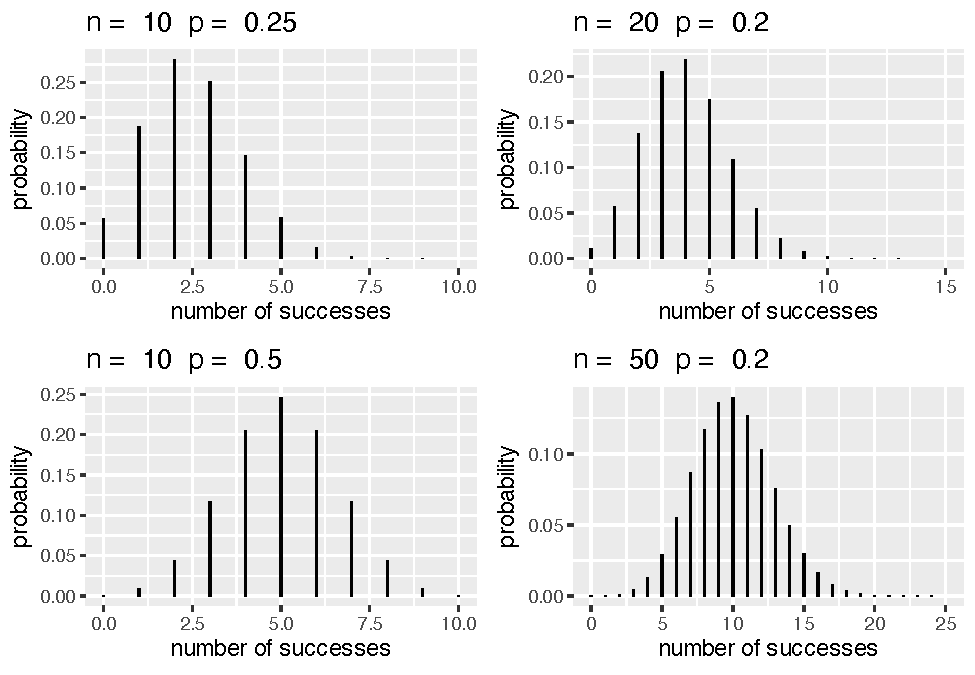
\includegraphics[width=0.6\linewidth]{bookdown-BeyondMLR_files/figure-latex/multBin-1} 

}

\caption{Binomial distributions with different values of \(n\) and \(p\).}\label{fig:multBin}
\end{figure}

\vspace{2cm}

Note that if \(n=1\),

\begin{align*}
 P(Y=y) &= \binom{1}{y} p^y(1-p)^{1-y} \\
        &= p^y(1-p)^{1-y}\quad \textrm{for}\quad y = 0, 1,
\end{align*}
a Bernoulli distribution! In fact, Bernoulli random variables are a special case of binomial random variables where \(n=1\).

In R we can use the function \texttt{dbinom(y,\ n,\ p)}, which outputs the probability of \(y\) successes given \(n\) trials with probability \(p\), i.e., \(P(Y=y)\) for \(Y \sim \textrm{Binomial}(n,p)\).

\textbf{Example 2:} While taking a multiple choice test, a student encountered 10 problems where she ended up completely guessing, randomly selecting one of the four options. What is the chance that she got exactly 2 of the 10 correct?

Knowing that the student randomly selected her answers, we assume she has a 25\% chance of a correct response. Thus, \(P(Y=2) = {10 \choose 2}(.25)^2(.75)^8 = 0.282\). We can use R to verify this:

\begin{Shaded}
\begin{Highlighting}[]
\KeywordTok{dbinom}\NormalTok{(}\DecValTok{2}\NormalTok{, }\DataTypeTok{size =} \DecValTok{10}\NormalTok{, }\DataTypeTok{prob =} \FloatTok{.25}\NormalTok{)}
\end{Highlighting}
\end{Shaded}

\begin{verbatim}
## [1] 0.2816
\end{verbatim}

Therefore, there is a 28\% chance of exactly 2 correct answers out of 10.

\hypertarget{geometric-random-variable}{%
\subsection{Geometric Random Variable}\label{geometric-random-variable}}

Suppose we are to perform independent, identical Bernoulli trials until the first success. If we wish to model \(Y\), the number of failures before the first success, we can consider the following pmf:

\begin{equation}
P(Y=y) = (1-p)^yp \quad \textrm{for}\quad y = 0, 1, \ldots, \infty.
\label{eq:geomRV}
\end{equation}

We can think about this function as modeling the probability of \(y\) failures, then 1 success. In this case, \(Y\) follows a \textbf{geometric distribution} \index{geometric distribution} with \(\E(Y) = \frac{1-p}p\) and \(\SD(Y) = \sqrt{\frac{1-p}{p^2}}\).



\begin{figure}

{\centering 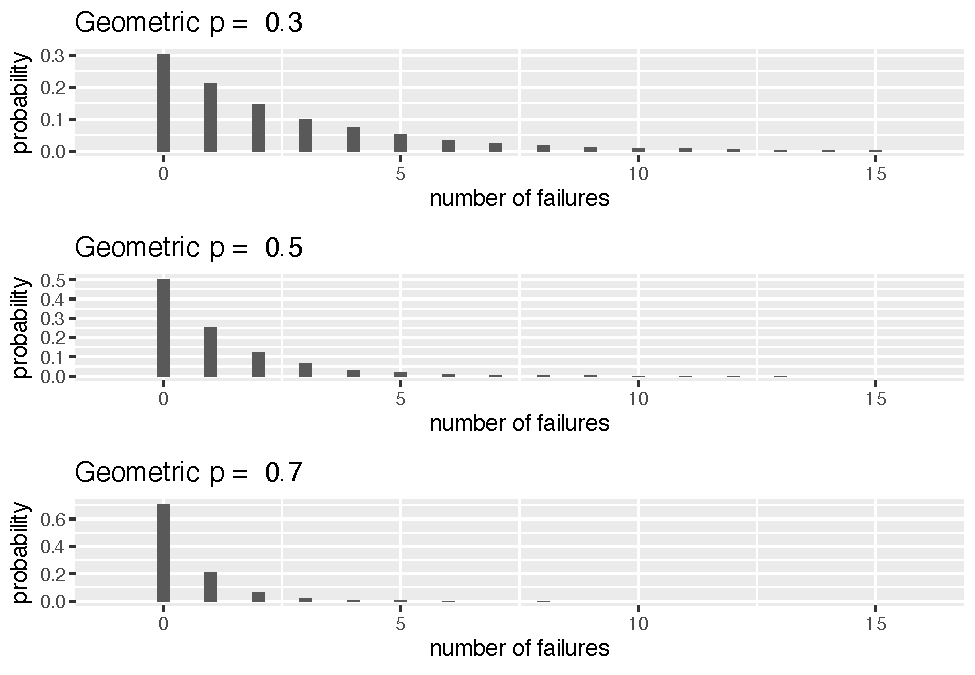
\includegraphics[width=0.6\linewidth]{bookdown-BeyondMLR_files/figure-latex/multGeo-1} 

}

\caption{Geometric distributions with \(p = 0.3,\ 0.5\) and \(0.7\).}\label{fig:multGeo}
\end{figure}

Typical shapes of geometric distributions are shown in Figure \ref{fig:multGeo}. Notice that as \(p\) increases, the range of plausible values decreases and means shift towards 0.

Once again, we can use R to aid our calculations. The function \texttt{dgeom(y,\ p)} will output the probability of \(y\) failures before the first success where \(Y \sim \textrm{Geometric}(p)\).

\textbf{Example 3:} Consider rolling a fair, six-sided die until a five appears. What is the probability of rolling the first five on the third roll?

First note that \(p = 1/6\). We are then interested in \(P(Y=2)\), as we would want 2 failures before our success. We know that \(P(Y=2) = (5/6)^2(1/6) = 0.116\). Verifying through R:

\begin{Shaded}
\begin{Highlighting}[]
\KeywordTok{dgeom}\NormalTok{(}\DecValTok{2}\NormalTok{, }\DataTypeTok{prob =} \DecValTok{1}\OperatorTok{/}\DecValTok{6}\NormalTok{)}
\end{Highlighting}
\end{Shaded}

\begin{verbatim}
## [1] 0.1157
\end{verbatim}

Thus, there is a 12\% chance of rolling the first five on the third roll.

\hypertarget{negative-binomial-random-variable}{%
\subsection{Negative Binomial Random Variable}\label{negative-binomial-random-variable}}

What if we were to carry out multiple independent and identical Bernoulli trails until the \(r\)\textsuperscript{th} success occurs?
If we model \(Y\), the number of failures before the \(r\)\textsuperscript{th} success, then \(Y\) follows a \textbf{negative binomial distribution} \index{negative binomial distribution} where

\begin{equation}
P(Y=y) = \binom{y + r - 1}{r-1} (1-p)^{y}(p)^r \quad \textrm{for}\quad y = 0, 1, \ldots, \infty.
\label{eq:nBinomRV}
\end{equation}
If \(Y \sim \textrm{Negative Binomial}(r, p)\) then \(\E(Y) = \frac{r(1-p)}{p}\) and \(\SD(Y) = \sqrt{\frac{r(1-p)}{p^2}}\). Figure \ref{fig:multNBinom} displays three negative binomial distributions. Notice how centers shift right as \(r\) increases, and left as \(p\) increases.



\begin{figure}

{\centering 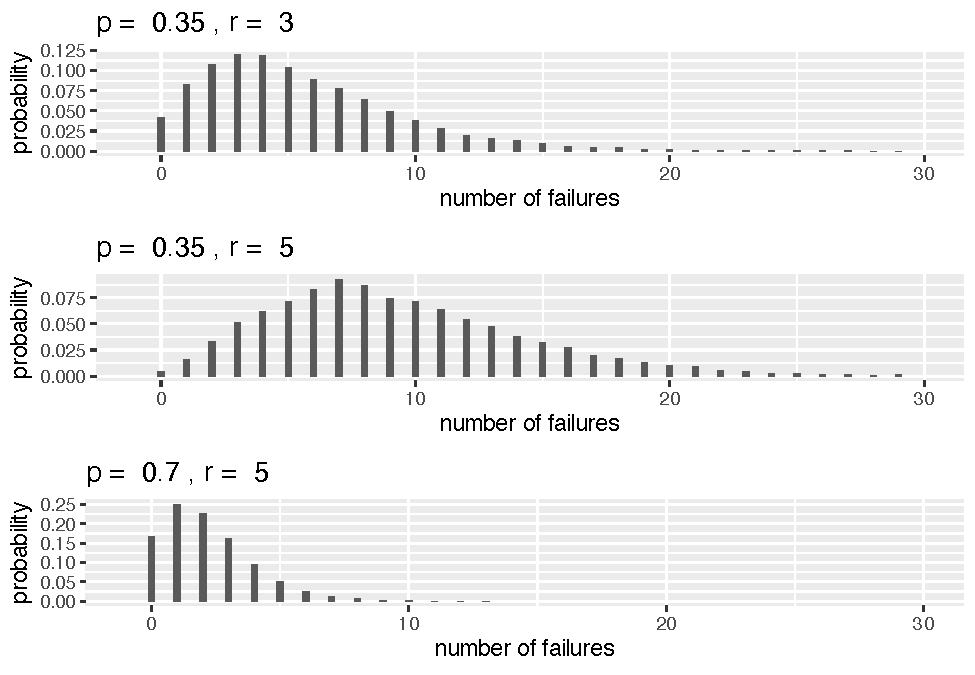
\includegraphics[width=0.6\linewidth]{bookdown-BeyondMLR_files/figure-latex/multNBinom-1} 

}

\caption{Negative binomial distributions with different values of \(p\) and \(r\).}\label{fig:multNBinom}
\end{figure}

Note that if we set \(r=1\), then

\begin{align*}
 P(Y=y) &= \binom{y}{0} (1-p)^yp \\
        &= (1-p)^yp \quad \textrm{for} \quad y = 0, 1, \ldots, \infty,
\end{align*}
which is the probability mass function of a geometric random variable! Thus, a geometric random variable is, in fact, a special case of a negative binomial random variable.

While negative binomial random variables typically are expressed as above using binomial coefficients (expressions such as \(\binom{x}{y}\)), we can generalize our definition to allow non-integer values of \(r\). This will come in handy later when modeling. To do this, we need to first introduce the \textbf{gamma function}. \index{gamma function} The gamma function is defined as such

\begin{equation}
\Gamma(x)  = \int_0^\infty t^{x-1} e^{-t}dt.
\label{eq:gammaFun}
\end{equation}
One important property of the gamma function is that for any integer \(n\), \(\Gamma(n) = (n-1)!\). Applying this, we can generalize the pmf of a negative binomial variable such that

\begin{align*}
 P(Y=y) &= \binom{y + r - 1}{r-1}           (1-p)^{y}(p)^r \\
        &= \frac{(y+r-1)!}{(r-1)!y!}         (1-p)^{y}(p)^r \\
        &= \frac{\Gamma(y+r)}{\Gamma(r) y!}  (1-p)^{y}(p)^r \quad \textrm{for} \quad y = 0, 1, \ldots, \infty.
\end{align*}
With this formulation, \(r\) is no longer restricted to non-negative integers; rather \(r\) can be any non-negative real number.

In R we can use the function \texttt{dnbinom(y,\ r,\ p)} for the probability of \(y\) failures before the \(r\)\textsuperscript{th} success given probability \(p\).

\textbf{Example 4:} A contestant on a game show needs to answer 10 questions correctly to win the jackpot. However, if they get 3 incorrect answers, they are kicked off the show. Suppose one contestant consistently has a 90\% chance of correctly responding to any question. What is the probability that she will correctly answer 10 questions before 3 incorrect responses?

Letting \(Y\) represent the number of incorrect responses, and setting \(r = 10\), we want

\begin{align*}
 P(Y < 3) &= P(Y=0) + P(Y=1) + P(Y=2) \\
          &= \binom{9}{9}(1-0.9)^0 (0.9)^{10} + \binom{10}{9}(1-0.9)^1 (0.9)^{10} \\
          & \quad + \binom{11}{9}(1-0.9)^2 (0.9)^{10} \\
          &= 0.89
\end{align*}
Using R:

\begin{Shaded}
\begin{Highlighting}[]
\CommentTok{# could also use pnbinom(2, 10, .9)}
\KeywordTok{sum}\NormalTok{(}\KeywordTok{dnbinom}\NormalTok{(}\DecValTok{0}\OperatorTok{:}\DecValTok{2}\NormalTok{, }\DataTypeTok{size =} \DecValTok{10}\NormalTok{, }\DataTypeTok{prob =} \FloatTok{.9}\NormalTok{))  }
\end{Highlighting}
\end{Shaded}

\begin{verbatim}
## [1] 0.8891
\end{verbatim}

Thus, there is a 89\% chance that she gets 10 correct responses before missing 3.

\hypertarget{hypergeometric-random-variable}{%
\subsection{Hypergeometric Random Variable}\label{hypergeometric-random-variable}}

In all previous random variables, we considered a Bernoulli process, where the probability of a success remained constant across all trials. What if this probability is dynamic? The \textbf{hypergeometric random variable} helps us address some of these situations. Specifically, what if we wanted to select \(n\) items \emph{without replacement} from a collection of \(N\) objects, \(m\) of which are considered successes? In that case, the probability of selecting a ``success'' depends on the previous selections.
If we model \(Y\), the number of successes after \(n\) selections, \(Y\) follows a \textbf{hypergeometric distribution} \index{hypergeometric distribution} where

\begin{equation}
P(Y=y) = \frac{\binom{m}{y} \binom{N-m}{n-y}}{\binom{N}{n}} \quad \textrm{for} \quad y = 0, 1, \ldots, \min(m,n).
\label{eq:hyperGeoRV}
\end{equation}

If \(Y\) follows a hypergeometric distribution and we define \(p = m/N\), then \(\E(Y) = np\) and \(\SD(Y) = \sqrt{np(1-p)\frac{N-n}{N-1}}\). Figure \ref{fig:multHyper} displays several hypergeometric distributions. On the left, \(N\) and \(n\) are held constant. As \(m \rightarrow N/2\), the distribution becomes more and more symmetric. On the right, \(m\) and \(N\) are held constant. Both distributions are displayed on the same scale. We can see that as \(n \rightarrow N\) (or \(n \rightarrow 0\)), the distribution becomes less variable.



\begin{figure}

{\centering 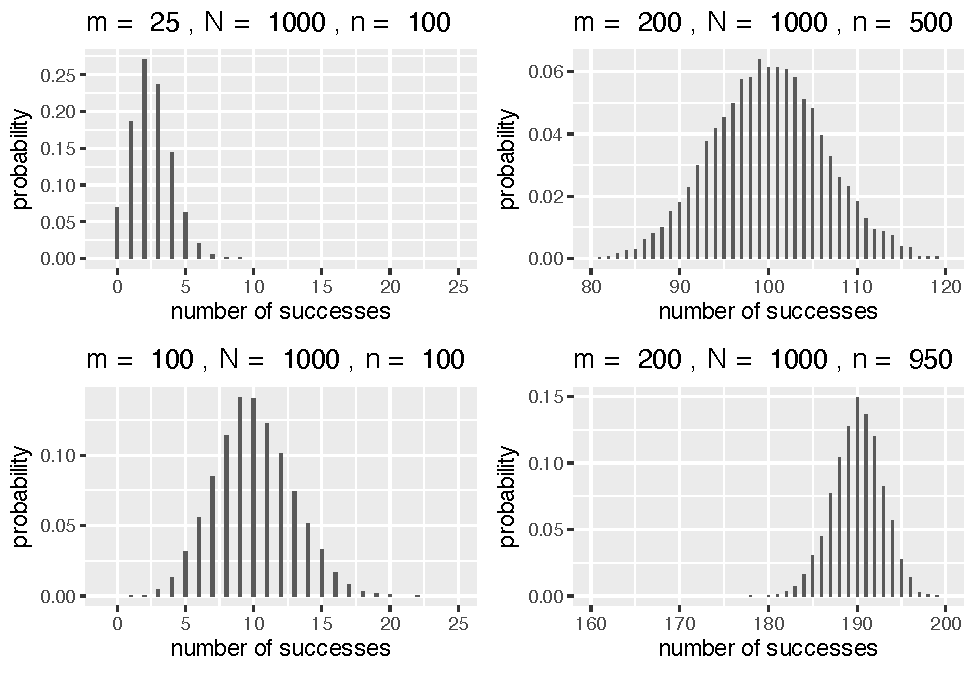
\includegraphics[width=0.6\linewidth]{bookdown-BeyondMLR_files/figure-latex/multHyper-1} 

}

\caption{Hypergeometric distributions with different values of \(m\), \(N\), and \(n\).}\label{fig:multHyper}
\end{figure}

If we wish to calculate probabilities through R, \texttt{dhyper(y,\ m,\ N-m,\ n)} gives \(P(Y=y)\) given \(n\) draws without replacement from \(m\) successes and \(N-m\) failures.

\textbf{Example 5:} Suppose a deck of cards is randomly shuffled. What is the probability that all 4 queens are located within the first 10 cards?

We can model \(Y\), the number of queens in the first 10 cards as a hypergeometric random variable where \(n = 10\), \(m = 4\), and \(N = 52\). Then, \(P(Y=4) = \displaystyle \frac{\binom{4}{4}\binom{48}{6}}{\binom{52}{10}} = 0.0008\). We can avoid this calculation through R, of course:

\begin{Shaded}
\begin{Highlighting}[]
\KeywordTok{dhyper}\NormalTok{(}\DecValTok{4}\NormalTok{, }\DataTypeTok{m =} \DecValTok{4}\NormalTok{, }\DataTypeTok{n =} \DecValTok{48}\NormalTok{, }\DataTypeTok{k =} \DecValTok{10}\NormalTok{)}
\end{Highlighting}
\end{Shaded}

\begin{verbatim}
## [1] 0.0007757
\end{verbatim}

So, there is a 0.08\% chance of all 4 queens being within the first 10 cards of a randomly shuffled deck of cards.

\hypertarget{poisson-random-variable}{%
\subsection{Poisson Random Variable}\label{poisson-random-variable}}

Sometimes, random variables are based on a \textbf{Poisson process}. \index{Poisson process} In a Poisson process, we are counting the number of events per unit of time or space and the number of events depends only on the length or size of the interval.
We can then model \(Y\), the number of events in one of these sections with the \textbf{Poisson distribution}, \index{Poisson distribution} where

\begin{equation}
P(Y=y) = \frac{e^{-\lambda}\lambda^y}{y!} \quad \textrm{for} \quad y = 0, 1, \ldots, \infty,
\label{eq:poissRV}
\end{equation}
where \(\lambda\) is the mean or expected count in the unit of time or space of interest.
This probability mass function has \(\E(Y) = \lambda\) and \(\SD(Y) = \sqrt{\lambda}\). Three Poisson distributions are displayed in Figure \ref{fig:multPois}. Notice how distributions become more symmetric as \(\lambda\) increases.



\begin{figure}

{\centering 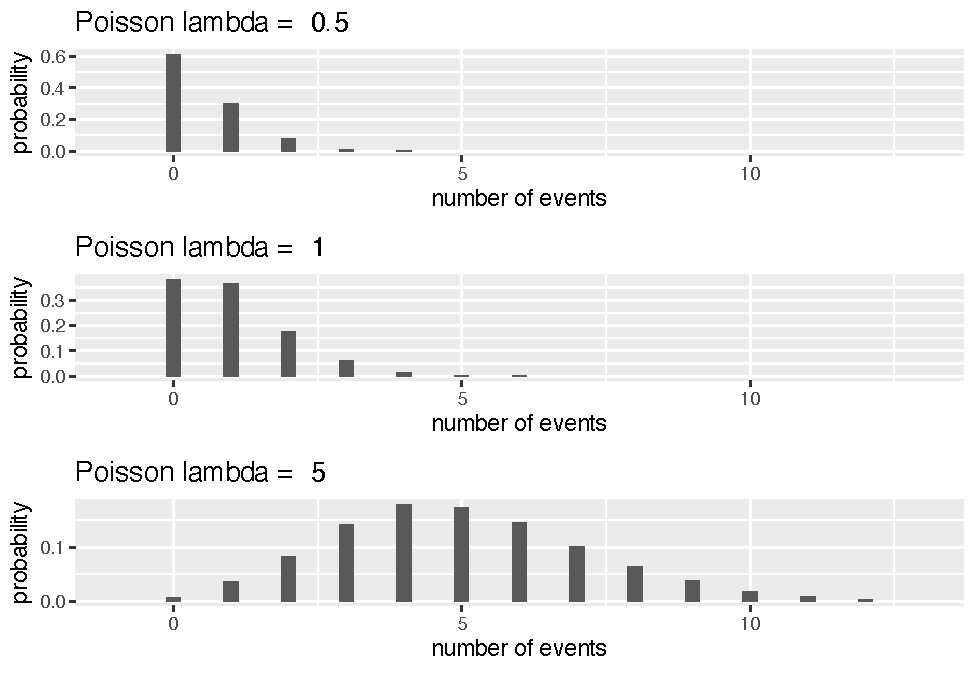
\includegraphics[width=0.6\linewidth]{bookdown-BeyondMLR_files/figure-latex/multPois-1} 

}

\caption{Poisson distributions with \(\lambda = 0.5,\ 1\), and \(5\).}\label{fig:multPois}
\end{figure}

If we wish to use R, \texttt{dpois(y,\ lambda)} outputs the probability of \(y\) events given \(\lambda\).

\textbf{Example 6:} A small town's police department issues 5 speeding tickets per month on average. Using a Poisson random variable, what is the likelihood that the police department issues 3 or fewer tickets in one month?

First, we note that here \(P(Y \le 3) = P(Y=0) + P(Y=1) + \cdots + P(Y=3)\). Applying the probability mass function for a Poisson distribution with \(\lambda = 5\), we find that

\begin{align*}
 P(Y \le 3) &= P(Y=0) + P(Y=1) + P(Y=2) + P(Y=3) \\
            &= \frac{e^{-5}5^0}{0!} + \frac{e^{-5}5^1}{1!} + \frac{e^{-5}5^2}{2!} + \frac{e^{-5}5^3}{3!}\\
            &= 0.27.
\end{align*}

We can verify through R:

\begin{Shaded}
\begin{Highlighting}[]
\KeywordTok{sum}\NormalTok{(}\KeywordTok{dpois}\NormalTok{(}\DecValTok{0}\OperatorTok{:}\DecValTok{3}\NormalTok{, }\DataTypeTok{lambda =} \DecValTok{5}\NormalTok{))   }\CommentTok{# or use ppois(3, 5)}
\end{Highlighting}
\end{Shaded}

\begin{verbatim}
## [1] 0.265
\end{verbatim}

Therefore, there is a 27\% chance of 3 or fewer tickets being issued within one month.

\hypertarget{continuous-random-variables}{%
\section{Continuous Random Variables}\label{continuous-random-variables}}

A continuous random variable can take on an uncountably infinite number of values. With continuous random variables, we define probabilities using \textbf{probability density functions} (pdfs). \index{probability density function (pdf)} Probabilities are calculated by computing the area under the density curve over the interval of interest. So, given a pdf, \(f(y)\), we can compute

\begin{align*}
P(a \le Y \le b) = \int_a^b f(y)dy.
\end{align*}
This hints at a few properties of continuous random variables:

\begin{itemize}
\tightlist
\item
  \(\int_{-\infty}^{\infty} f(y)dy = 1\).\\
\item
  For any value \(y\), \(P(Y = y) = \int_y^y f(y)dy = 0\).\\
\item
  Because of the above property, \(P(y < Y) = P(y \le Y)\). We will typically use the first notation rather than the second, but both are equally valid.
\end{itemize}

\hypertarget{exponential-random-variable}{%
\subsection{Exponential Random Variable}\label{exponential-random-variable}}

Suppose we have a Poisson process with rate \(\lambda\), and we wish to model the wait time \(Y\) until the first event. We could model \(Y\) using an \textbf{exponential distribution}, \index{exponential distribution} where

\begin{equation}
f(y) = \lambda e^{-\lambda y} \quad \textrm{for} \quad y > 0,
\label{eq:expRV}
\end{equation}
where \(\E(Y) = 1/\lambda\), \(\SD(Y) = 1/\lambda\). Figure \ref{fig:multExp} displays three exponential distributions with different \(\lambda\) values. As \(\lambda\) increases, \(\E(Y)\) tends towards 0, and distributions ``die off'' quicker.



\begin{figure}

{\centering 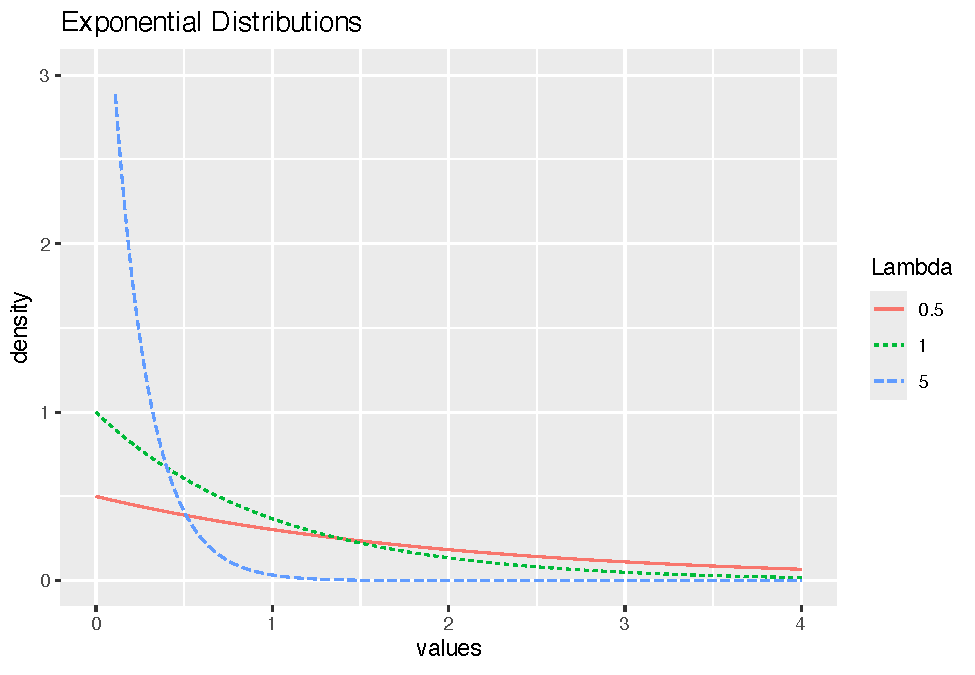
\includegraphics[width=0.6\linewidth]{bookdown-BeyondMLR_files/figure-latex/multExp-1} 

}

\caption{Exponential distributions with \(\lambda = 0.5, 1,\) and \(5\).}\label{fig:multExp}
\end{figure}

If we wish to use R, \texttt{pexp(y,\ lambda)} outputs the probability \(P(Y < y)\) given \(\lambda\).

\textbf{Example 7:} Refer to Example 6. What is the probability that 10 days or fewer elapse between two tickets being issued?

We know the town's police issue 5 tickets per month. For simplicity's sake, assume each month has 30 days. Then, the town issues \(\frac{1}{6}\) tickets per day. That is \(\lambda = \frac{1}{6}\), and the average wait time between tickets is \(\frac{1}{1/6} = 6\) days. Therefore,

\begin{align*}
P(Y < 10) = \int_{0}^{10} \textstyle \frac16 e^{-\frac16y} dy = 0.81.
\end{align*}

We can also use R:

\begin{Shaded}
\begin{Highlighting}[]
\KeywordTok{pexp}\NormalTok{(}\DecValTok{10}\NormalTok{, }\DataTypeTok{rate =} \DecValTok{1}\OperatorTok{/}\DecValTok{6}\NormalTok{)}
\end{Highlighting}
\end{Shaded}

\begin{verbatim}
## [1] 0.8111
\end{verbatim}

Hence, there is a 81\% chance of waiting fewer than 10 days between tickets.

\hypertarget{gamma-random-variable}{%
\subsection{Gamma Random Variable}\label{gamma-random-variable}}

Once again consider a Poisson process. When discussing exponential random variables, we modeled the wait time before one event occurred. If \(Y\) represents the wait time before \(r\) events occur in a Poisson process with rate \(\lambda\), \(Y\) follows a \textbf{gamma distribution} \index{gamma distribution} where

\begin{equation}
f(y) = \frac{\lambda^r}{\Gamma(r)} y^{r-1} e^{-\lambda y}\quad \textrm{for} \quad y >0.
\label{eq:gammaRV}
\end{equation}

If \(Y \sim \textrm{Gamma}(r, \lambda)\) then \(\E(Y) = r/\lambda\) and \(\SD(Y) = \sqrt{r/\lambda^2}\). A few gamma distributions are displayed in Figure \ref{fig:multGamma}. Observe that means increase as \(r\) increases, but decrease as \(\lambda\) increases.



\begin{figure}

{\centering 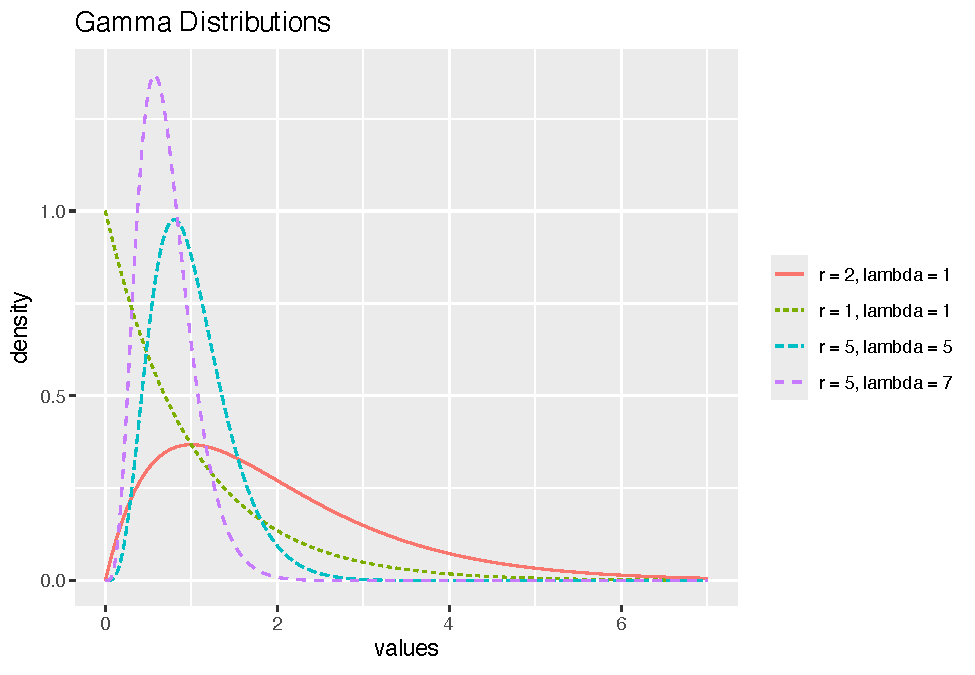
\includegraphics[width=0.6\linewidth]{bookdown-BeyondMLR_files/figure-latex/multGamma-1} 

}

\caption{Gamma distributions with different values of \(r\) and \(\lambda\).}\label{fig:multGamma}
\end{figure}

Note that if we let \(r = 1\), we have the following pdf,

\begin{align*}
 f(y) &= \frac{\lambda}{\Gamma(1)} y^{1-1} e^{-\lambda y} \\
      &= \lambda e^{-\lambda y} \quad \textrm{for} \quad y > 0,
\end{align*}
an exponential distribution. Just as how the geometric distribution was a special case of the negative binomial, exponential distributions are in fact a special case of gamma distributions!

Just like negative binomial, the pdf of a gamma distribution is defined for all real, non-negative \(r\).

In R, \texttt{pgamma(y,\ r,\ lambda)} outputs the the probability \(P(Y < y)\) given \(r\) and \(\lambda\).

\textbf{Example 8:} Two friends are out fishing. On average they catch two fish per hour, and their goal is to catch 5 fish. What is the probability that they take less than 3 hours to reach their goal?

Using a gamma random variable, we set \(r = 5\) and \(\lambda = 2\). So,

\begin{align*}
P(Y < 3) = \int_0^3 \frac{2^4}{\Gamma(5)} y^{4} e^{-2y}dy = 0.715.
\end{align*}

Using R:

\begin{Shaded}
\begin{Highlighting}[]
\KeywordTok{pgamma}\NormalTok{(}\DecValTok{3}\NormalTok{, }\DataTypeTok{shape =} \DecValTok{5}\NormalTok{, }\DataTypeTok{rate =} \DecValTok{2}\NormalTok{)}
\end{Highlighting}
\end{Shaded}

\begin{verbatim}
## [1] 0.7149
\end{verbatim}

There is a 71.5\% chance of catching 5 fish within the first 3 hours.

\hypertarget{normal-gaussian-random-variable}{%
\subsection{Normal (Gaussian) Random Variable}\label{normal-gaussian-random-variable}}

You have already at least informally seen normal random variables when evaluating LLSR assumptions. To recall, we required responses to be normally distributed at each level of \(X\). Like any continuous random variable, normal (also called Gaussian) random variables have their own pdf, dependent on \(\mu\), the population mean of the variable of interest, and \(\sigma\), the population standard deviation. We find that

\begin{equation}
f(y) =  \frac{e^{-(y-\mu)^2/ (2 \sigma^2)}}{\sqrt{2\pi\sigma^2}} \quad \textrm{for} \quad -\infty < y < \infty.
\label{eq:normalRV}
\end{equation}

As the parameter names suggest, \(\E(Y) = \mu\) and \(\SD(Y) = \sigma\). Often, normal distributions are referred to as \(\textrm{N}(\mu, \sigma)\), implying a normal distribution \index{normal distribution} with mean \(\mu\) and standard deviation \(\sigma\). The distribution \(\textrm{N}(0,1)\) is often referred to as the \textbf{standard normal distribution}. A few normal distributions are displayed in Figure \ref{fig:multNorm}.



\begin{figure}

{\centering 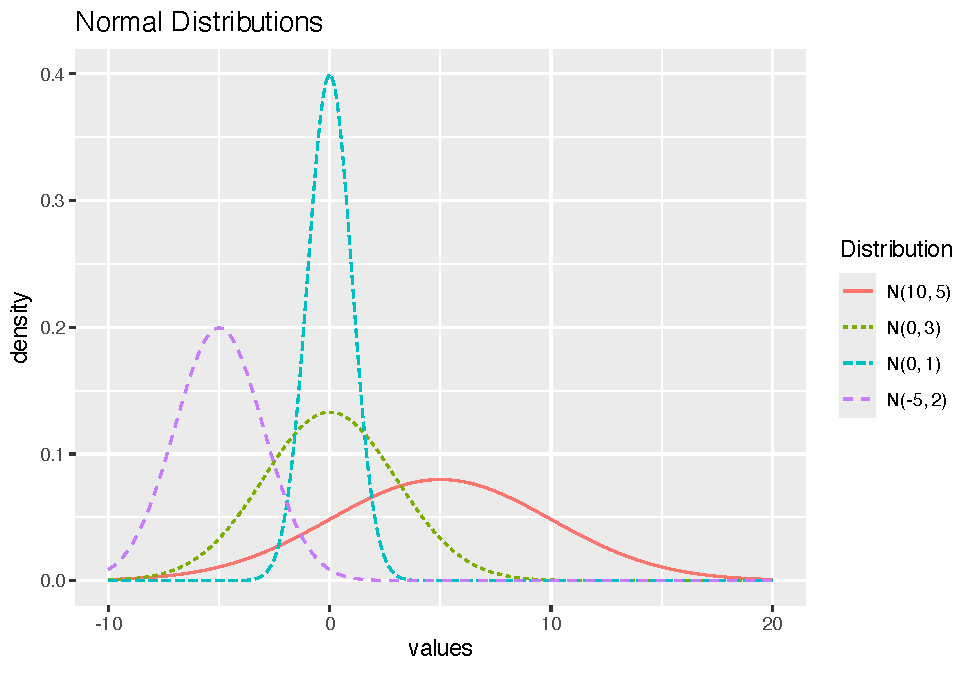
\includegraphics[width=0.6\linewidth]{bookdown-BeyondMLR_files/figure-latex/multNorm-1} 

}

\caption{Normal distributions with different values of \(\mu\) and \(\sigma\).}\label{fig:multNorm}
\end{figure}

In R, \texttt{pnorm(y,\ mean,\ sd)} outputs the probability \(P(Y < y)\) given a mean and standard deviation.

\textbf{Example 9:} The weight of a box of Fruity Tootie cereal is approximately normally distributed with an average weight of 15 ounces and a standard deviation of 0.5 ounces. What is the probability that the weight of a randomly selected box is more than 15.5 ounces?

Using a normal distribution,

\begin{align*} 
P(Y > 15.5) = \int_{15.5}^{\infty} \frac{e^{-(y-15)^2/ (2\cdot 0.5^2)}}{\sqrt{2\pi\cdot 0.5^2}}dy = 0.159
\end{align*}

We can use R as well:

\begin{Shaded}
\begin{Highlighting}[]
\KeywordTok{pnorm}\NormalTok{(}\FloatTok{15.5}\NormalTok{, }\DataTypeTok{mean =} \DecValTok{15}\NormalTok{, }\DataTypeTok{sd =} \FloatTok{0.5}\NormalTok{, }\DataTypeTok{lower.tail =} \OtherTok{FALSE}\NormalTok{)}
\end{Highlighting}
\end{Shaded}

\begin{verbatim}
## [1] 0.1587
\end{verbatim}

There is a 16\% chance of a randomly selected box weighing more than 15.5 ounces.

\hypertarget{beta-random-variable}{%
\subsection{Beta Random Variable}\label{beta-random-variable}}

So far, all of our continuous variables have had no upper bound. If we want to limit our possible values to a smaller interval, we may turn to a \textbf{beta random variable}. In fact, we often use beta random variables to model distributions of probabilities---bounded below by 0 and above by 1. The pdf is parameterized by two values, \(\alpha\) and \(\beta\) (\(\alpha, \beta > 0\)). We can describe a beta random variable by the following pdf:

\begin{equation}
f(y) = \frac{\Gamma(\alpha + \beta)}{\Gamma(\alpha)\Gamma(\beta)} y^{\alpha-1} (1-y)^{\beta-1} \quad \textrm{for} \quad 0 < y < 1.
\label{eq:betaRV}
\end{equation}

If \(Y \sim \textrm{Beta}(\alpha, \beta)\), then \(\E(Y) = \alpha/(\alpha + \beta)\) and \(\SD(Y) = \displaystyle \sqrt{\frac{\alpha \beta}{(\alpha + \beta)^2 (\alpha+\beta+1)}}\). Figure \ref{fig:multBeta} displays several beta distributions. \index{beta distribution} Note that when \(\alpha = \beta\), distributions are symmetric. The distribution is left-skewed when \(\alpha > \beta\) and right-skewed when \(\beta > \alpha\).



\begin{figure}

{\centering 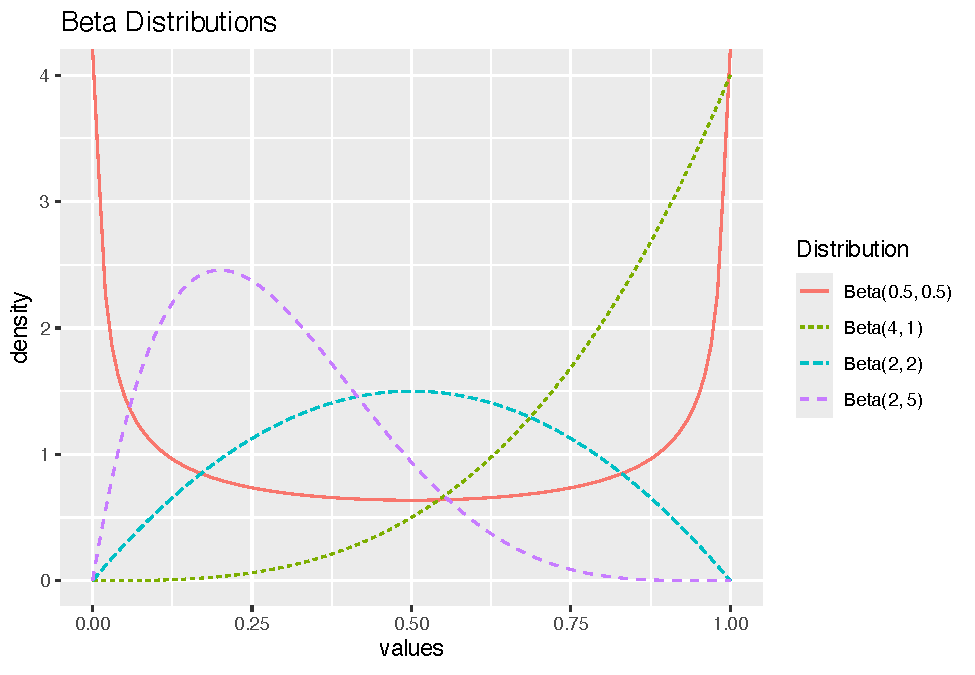
\includegraphics[width=0.6\linewidth]{bookdown-BeyondMLR_files/figure-latex/multBeta-1} 

}

\caption{Beta distributions with different values of \(\alpha\) and \(\beta\).}\label{fig:multBeta}
\end{figure}

If \(\alpha = \beta = 1\), then

\begin{align*}
 f(y) &= \frac{\Gamma(1)}{\Gamma(1)\Gamma(1)}y^0(1-y)^0 \\
      &= 1 \quad \textrm{for} \quad 0 < y < 1.
\end{align*}
This distribution is referred to as a \textbf{uniform distribution}.

In R, \texttt{pbeta(y,\ alpha,\ beta)} yields \(P(Y < y)\) assuming \(Y \sim \textrm{Beta}(\alpha, \beta)\).

\textbf{Example 10:} A private college in the Midwest models the probabilities of prospective students accepting an admission decision through a beta distribution with \(\alpha = \frac{4}{3}\) and \(\beta = 2\). What is the probability that a randomly selected student has probability of accepting greater than 80\%?

Letting \(Y \sim \textrm{Beta}(4/3,2)\), we can calculate

\begin{align*} 
P(Y > 0.8) = \int_{0.8}^1 \frac{\Gamma(4/3 + 2)}{\Gamma(4/3)\Gamma(2)} y^{4/3-1} (1-y)^{2-1}dy = 0.06.
\end{align*}

Alternatively, in R:

\begin{Shaded}
\begin{Highlighting}[]
\KeywordTok{pbeta}\NormalTok{(}\FloatTok{0.8}\NormalTok{, }\DataTypeTok{shape1 =} \DecValTok{4}\OperatorTok{/}\DecValTok{3}\NormalTok{, }\DataTypeTok{shape2 =} \DecValTok{2}\NormalTok{, }\DataTypeTok{lower.tail =} \OtherTok{FALSE}\NormalTok{)}
\end{Highlighting}
\end{Shaded}

\begin{verbatim}
## [1] 0.0593
\end{verbatim}

Hence, there is a 6\% chance that a randomly selected student has a probability of accepting an admission decision above 80\%.

\hypertarget{distributions-used-in-testing}{%
\section{Distributions Used in Testing}\label{distributions-used-in-testing}}

We have spent most of this chapter discussing probability distributions that may come in handy when modeling. The following distributions, while rarely used in modeling, prove useful in hypothesis testing as certain commonly used test statistics follow these distributions.

\hypertarget{chi2-distribution}{%
\subsection{\texorpdfstring{\(\chi^2\) Distribution}{\textbackslash chi\^{}2 Distribution}}\label{chi2-distribution}}

You have probably already encountered \(\chi^2\) tests before. For example, \(\chi^2\) tests are used with two-way contingency tables to investigate the association between row and column variables. \(\chi^2\) tests are also used in goodness-of-fit testing such as comparing counts expected according to Mendelian ratios to observed data. In those situations, \(\chi^2\) tests compare observed counts to what would be expected under the null hypotheses and reject the null when these observed discrepancies are too large.

In this course, we encounter \(\chi^2\) distributions \index{chi-square distribution} in several testing situations. In Section \ref{sec-lrtest} we performed likelihood ratio tests (LRTs) to compare nested models. When a larger model provides no significant improvement over a reduced model, the LRT statistic (which is twice the difference in the log-likelihoods) follows a \(\chi^2\) distribution with the degrees of freedom equal to the difference in the number of parameters.

In general, \(\chi^2\) distributions with \(k\) degrees of freedom are right skewed with a mean \(k\) and standard deviation \(\sqrt{2k}\). Figure \ref{fig:multChisq} displays chi-square distributions with different values of \(k\).

The \(\chi^2\) distribution is a special case of gamma distributions. Specifically, a \(\chi^2\) distribution with \(k\) degrees of freedom can be expressed as a gamma distribution with \(\lambda = 1/2\) and \(r = k/2\).



\begin{figure}

{\centering 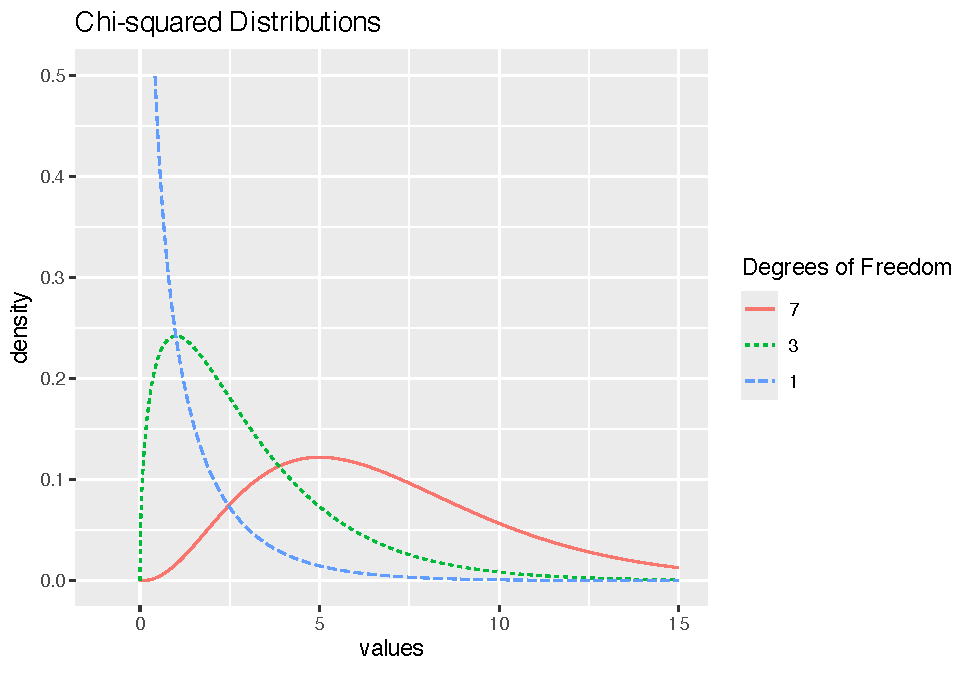
\includegraphics[width=0.6\linewidth]{bookdown-BeyondMLR_files/figure-latex/multChisq-1} 

}

\caption{\(\chi^2\) distributions with 1, 3, and 7 degrees of freedom..}\label{fig:multChisq}
\end{figure}

In R, \texttt{pchisq(y,\ df)} outputs \(P(Y < y)\) given \(k\) degrees of freedom.

\hypertarget{students-t-distribution}{%
\subsection{\texorpdfstring{Student's \(t\)-Distribution}{Student's t-Distribution}}\label{students-t-distribution}}

You likely have seen Student's \(t\)-distribution \index{t distribution} (developed by William Sealy Gosset under the penname \emph{Student}) in a previous statistics course. You may have used it when drawing inferences about the means of normally distributed populations with unknown population standard deviations. \(t\)-distributions are parameterized by their degrees of freedom, \(k\).

A \(t\)-distribution with \(k\) degrees of freedom has mean \(0\) and standard deviation \(k/(k-2)\) (standard deviation is only defined for \(k > 2\)). As \(k \rightarrow \infty\) the \(t\)-distribution approaches the standard normal distribution.



\begin{figure}

{\centering 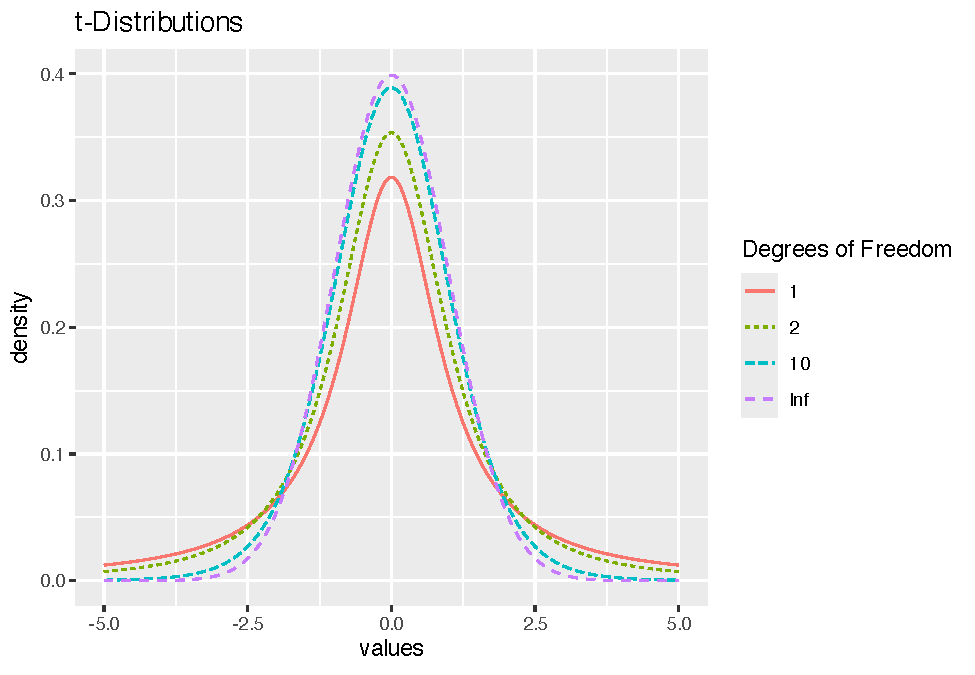
\includegraphics[width=0.6\linewidth]{bookdown-BeyondMLR_files/figure-latex/multT-1} 

}

\caption{\(t\)-distributions with 1, 2, 10, and Infinite degrees of freedom.}\label{fig:multT}
\end{figure}

Figure \ref{fig:multT} displays some \(t\)-distributions, where a \(t\)-distribution with infinite degrees of freedom is equivalent to a standard normal distribution (with mean 0 and standard deviation 1). In R, \texttt{pt(y,\ df)} outputs \(P(Y < y)\) given \(k\) degrees of freedom.

\hypertarget{f-distribution}{%
\subsection{\texorpdfstring{\(F\)-Distribution}{F-Distribution}}\label{f-distribution}}

\(F\)-distributions \index{F distribution} are also used when performing statistical tests. Like the \(\chi^2\) distribution, the values from an \(F\)-distribution are non-negative and the distribution is right skewed; in fact, an \(F\)-distribution can be derived as the ratio of two \(\chi^2\) random variables. R.A. Fisher (for whom the test is named) devised this test statistic to compare two different estimates of the same variance parameter, and it has a prominent role in Analysis of Variance (ANOVA). Model comparisons are often based on the comparison of variance estimates, e.g., the extra sums-of-squares \(F\) test. \(F\)-distributions are indexed by two degrees-of-freedom values, one for the numerator (\(k_1\)) and one for the denominator (\(k_2\)). The expected value for an \(F\)-distribution with \(k_1, k_2\) degrees of freedom under the null hypothesis is \(\frac{k_2}{k_2 - 2}\), which approaches \(1\) as \(k_2 \rightarrow \infty\). The standard deviation decreases as \(k_1\) increases for fixed \(k_2\), as seen in Figure \ref{fig:multF}, which illustrates several F-distributions.



\begin{figure}

{\centering 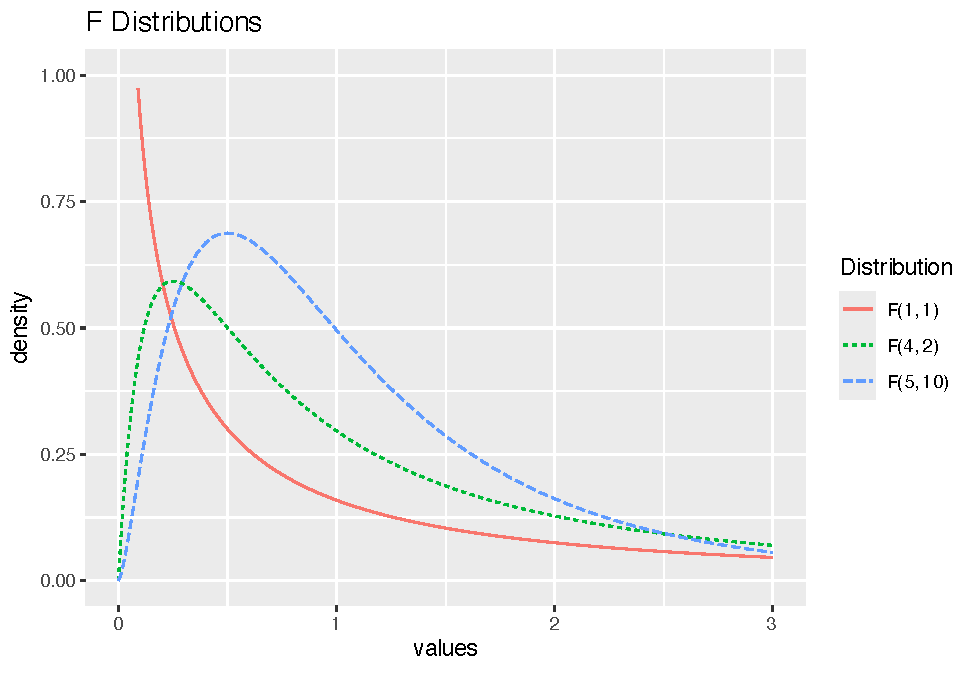
\includegraphics[width=0.6\linewidth]{bookdown-BeyondMLR_files/figure-latex/multF-1} 

}

\caption{\(F\)-distributions with different degrees of freedom.}\label{fig:multF}
\end{figure}

\hypertarget{additional-resources}{%
\section{Additional Resources}\label{additional-resources}}

Table \ref{tab:distTable} briefly details most of the random variables discussed in this chapter.

\begin{table}

\caption{\label{tab:distTable}Review of Mentioned Random Variables}
\centering
\resizebox{\linewidth}{!}{
\begin{tabular}[t]{llll>{\raggedright\arraybackslash}p{10em}}
\toprule
Distribution Name & pmf / pdf & Parameters & Possible Y Values & Description\\
\midrule
Binomial & ${n \choose y} p^y (1-p)^{n-y}$ & $p,\ n$ & $0, 1, \ldots , n$ & Number of successes after $n$ trials\\
Geometric & $(1-p)^yp$ & $p$ & $0, 1, \ldots, \infty$ & Number of failures until the first success\\
Negative Binomial & ${y + r - 1\choose r-1} (1-p)^{y}(p)^r$ & $p,\ r$ & $0, 1, \ldots, \infty$ & Number of failures before $r$ successes\\
Hypergeometric & ${m \choose y}{N-m \choose n-y}\big/{N \choose n}$ & $n,\ m,\ N$ & $0, 1, \ldots , \min(m,n)$ & Number of successes after $n$ trials without replacement\\
Poisson & ${e^{-\lambda}\lambda^y}\big/{y!}$ & $\lambda$ & $0, 1, \ldots, \infty$ & Number of events in a fixed interval\\
\addlinespace
Exponential & $\lambda e^{-\lambda y}$ & $\lambda$ & $(0, \infty)$ & Wait time for one event in a Poisson process\\
Gamma & $\displaystyle\frac{\lambda^r}{\Gamma(r)} y^{r-1} e^{-\lambda y}$ & $\lambda, \ r$ & $(0, \infty)$ & Wait time for $r$ events in a Poisson process\\
Normal & $\displaystyle\frac{e^{-(y-\mu)^2/ (2 \sigma^2)}}{\sqrt{2\pi\sigma^2}}$ & $\mu,\ \sigma$ & $(-\infty,\ \infty)$ & Used to model many naturally occurring phenomena\\
Beta & $\frac{\Gamma(\alpha + \beta)}{\Gamma(\alpha)\Gamma(\beta)} y^{\alpha-1} (1-y)^{\beta-1}$ & $\alpha,\ \beta$ & $(0,\ 1)$ & Useful for modeling probabilities\\
\bottomrule
\end{tabular}}
\end{table}

\hypertarget{exercises}{%
\section{Exercises}\label{exercises}}

\hypertarget{conceptual-exercises}{%
\subsection{Conceptual Exercises}\label{conceptual-exercises}}

\begin{enumerate}
\def\labelenumi{\arabic{enumi}.}
\item
  At what value of \(p\) is the standard deviation of a binary random variable smallest? When is standard deviation largest?
\item
  How are hypergeometric and binomial random variables different? How are they similar?
\item
  How are exponential and Poisson random variables related?
\item
  How are geometric and exponential random variables similar? How are they different?
\item
  A university's college of sciences is electing a new board of 5 members. There are 35 applicants, 10 of which come from the math department. What distribution could be helpful to model the probability of electing \(X\) board members from the math department?
\item
  Chapter 1 asked you to consider a scenario where \emph{``The Minnesota Pollution Control Agency is interested in using traffic volume data to generate predictions of particulate distributions as measured in counts per cubic feet.''} What distribution might be useful to model this count per cubic foot? Why?
\item
  Chapter 1 also asked you to consider a scenario where \emph{``Researchers are attempting to see if socioeconomic status and parental stability are predictive of low birthweight. They classify a low birthweight as below 2500 g, hence our response is binary: 1 for low birthweight, and 0 when the birthweight is not low.''} What distribution might be useful to model if a newborn has low birthweight?
\item
  Chapter 1 also asked you to consider a scenario where \emph{``Researchers are interested in how elephant age affects mating patterns among males. In particular, do older elephants have greater mating success, and is there an optimal age for mating among males? Data collected includes, for each elephant, age and number of matings in a given year.''} Which distribution would be useful to model the number of matings in a given year for these elephants? Why?
\item
  Describe a scenario which could be modeled using a gamma distribution.
\end{enumerate}

\hypertarget{guided-exercises}{%
\subsection{Guided Exercises}\label{guided-exercises}}

\begin{enumerate}
\def\labelenumi{\arabic{enumi}.}
\item
  \textbf{Beta-Binomial Distribution.} We can generate more distributions by mixing two random variables. \index{mixture model} Beta-binomial random variables are binomial random variables with fixed \(n\) whose parameter \(p\) follows a beta distribution with fixed parameters \(\alpha, \beta\). In more detail, we would first draw \(p_1\) from our beta distribution, and then generate our first observation \(y_1\), a random number of successes from a binomial (\(n, p_1\)) distribution. Then, we would generate a new \(p_2\) from our beta distribution, and use a binomial distribution with parameters \(n, p_2\) to generate our second observation \(y_2\). We would continue this process until desired.

  Note that all of the observations \(y_i\) will be integer values from \(0, 1, \ldots, n\). With this in mind, use \texttt{rbinom()} to simulate 1,000 observations from a plain old vanilla binomial random variable with \(n=10\) and \(p=0.8\). Plot a histogram of these binomial observations. Then, do the following to generate a beta-binomial distribution:

  \begin{enumerate}
  \def\labelenumii{\alph{enumii}.}
  \tightlist
  \item
    Draw \(p_i\) from the beta distribution with \(\alpha=4\) and \(\beta=1\).
  \item
    Generate an observation \(y_i\) from a binomial distribution with \(n=10\) and \(p = p_i\).
  \item
    Repeat (a) and (b) 1,000 times (\(i=1,\ldots,1000\)).
  \item
    Plot a histogram of these beta-binomial observations.
  \end{enumerate}

  Compare the histograms of the ``plain old'' binomial and beta-binomial distributions. How do their shapes, standard deviations, means, possible values, etc. compare?
\item
  \textbf{Gamma-Poisson Mixture I} Use the R function \texttt{rpois()} to generate 10,000 \(x_i\) from a plain old vanilla Poisson random variable, \(X \sim \textrm{Poisson}(\lambda=1.5)\). Plot a histogram of this distribution and note its mean and standard deviation. Next, let \(Y \sim \textrm{Gamma}(r = 3, \lambda = 2)\) and use \texttt{rgamma()} to generate 10,000 random \(y_i\) from this distribution. Now, consider 10,000 different Poisson distributions where \(\lambda_i = y_i\). Randomly generate one \(z_i\) from each Poisson distribution. Plot a histogram of these \(z_i\) and compare it to your original histogram of \(X\) (where \(X \sim \textrm{Poisson}(1.5)\)). How do the means and standard deviations compare?
\item
  \textbf{Gamma-Poisson Mixture II} A negative binomial distribution can actually be expressed as a gamma-Poisson mixture.
  In the previous problem's gamma-Poisson mixture \(Z \sim \textrm{Poisson}(\lambda)\) where \(\lambda \sim \textrm{Gamma}(r = 3, \lambda' = 2)\).
  Find the parameters of a negative binomial distribution \(X \sim \textrm{Negative Binomial}(r, p)\) such that \(X\) is equivalent to \(Z\). As a hint, the means of both distributions must be the same, so \(r(1-p)/p = 3/2\). Show through histograms and summary statistics that your negative binomial distribution is equivalent to your gamma-Poisson mixture from Problem 2. Argue that if you want a NB(\(r\), \(p\)) random variable, you can instead sample from a Poisson distribution, where the \(\lambda\) values are themselves sampled from a gamma distribution with parameters \(r\) and \(\lambda' = \frac{p}{1-p}\).
\item
  \textbf{Mixture of Two Normal Distributions} Sometimes, a value may be best modeled by a mixture of two normal distributions. We would have 5 parameters in this case--- \(\mu_1, \sigma_1, \mu_2, \sigma_2, \alpha\), where \(0 < \alpha < 1\) is a mixing parameter determining the probability that an observation comes from the first distribution. We would then have \(f(y) = \alpha\ f_1(y) + (1-\alpha)\ f_2(y)\) (where \(f_i(y)\) is the pdf of the normal distribution with \(\mu_i, \sigma_i\)). One phenomenon which could be modeled this way would be the waiting times between eruptions of Old Faithful geyser in Yellowstone National Park. The data can be accessed in R through \texttt{faithful}, and a histogram of wait times can be found in Figure \ref{fig:faithful}. The MLEs of our 5 parameters would be the combination of values that produces the maximum probability of our observed data. We will try to approximate MLEs by hand. Find a combination of \(\mu_1, \sigma_1, \mu_2, \sigma_2, \alpha\) for this distribution such that the logged likelihood is above -1050. (The command \texttt{dnorm(x,\ mean,\ sd)}, which outputs \(f(y)\) assuming \(Y \sim \textrm{N}(\mu, \sigma)\), will be helpful in calculating likelihoods.)
\end{enumerate}

\begin{figure}

{\centering 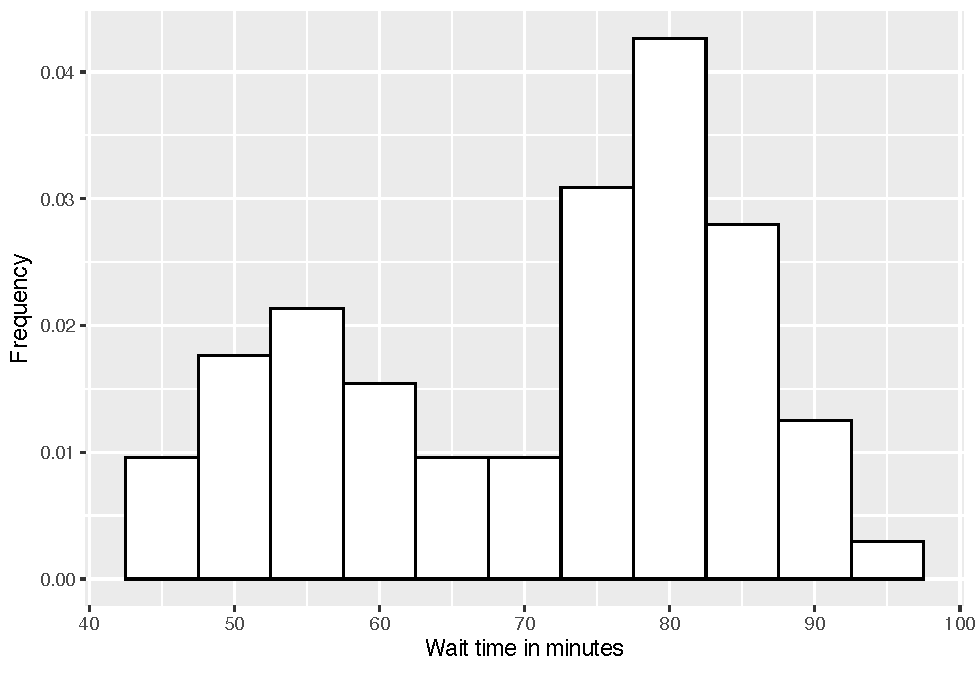
\includegraphics[width=0.6\linewidth]{bookdown-BeyondMLR_files/figure-latex/faithful-1} 

}

\caption{Waiting time between eruptions of Old Faithful.}\label{fig:faithful}
\end{figure}

  \bibliography{bib/articles.bib,bib/books.bib,bib/misc.bib}

\backmatter
\printindex

\end{document}
